%
%  order report template
%
%  Created by Matthias Laug on 2009-08-06.
%
\documentclass[a4paper]{article}


\renewcommand{\baselinestretch}{1.3}

% set font to times
\usepackage{mathptmx}
\usepackage[scaled=1]{helvet}

\renewcommand\familydefault{phv}

% set margins 
\usepackage[left=20mm, right=20mm, top=20mm, bottom=40mm] {geometry}

% Use utf-8 encoding for foreign characters
%\usepackage[applemac]{inputenc}
\usepackage[utf8]{inputenc}

% Use german language
\usepackage[german]{babel}

% Setup for fullpage use
% multirow - rowspan in tables
% graphicx - include graphics
% fancyhdr - footer/header
% booktabs - nice tables
\usepackage{multirow, graphicx, fancyhdr, booktabs,array,colortbl}

% define \EUR{amount}
\usepackage[right]{eurosym}

%booktabs settings
\newcolumntype{V}[1]{
	 >{\bfseries\huge}p{#1}
} 							% tabellen�berschriften
\newcolumntype{T}[1]{
	>{\bfseries\large}p{#1}
} 							% tabellen�berschriften
\newcolumntype{v}[1]{
	>{\raggedright}p{#1}
} 							% verwende v{Xcm} f�r linksb�ndige Spalten fester Breite
\newcolumntype{w}[1]{
	>{\raggedleft}p{#1}
} 							% verwende w{Xcm} f�r rechtsb�ndige Spalten fester Breite
\newcolumntype{x}[1]{
	>{\centering}p{#1}
} 							% verwende x{Xcm} f�r zentrierte Spalten fester Breite

% Define user colors using the RGB model
	\definecolor{black}{rgb}{0,0,0}

%-------------------------------- Kopf- und Fuzeile
\pagestyle{fancy}
\fancyhf{}
\setlength{\parindent}{0pt} 
%header
%\fancyhead[C]{
\includegraphics[scale=0.5]{../pdf/header_check.jpg}}
%\fancyhead[C]{
\includegraphics[scale=0.5]{../pdf/header.eps}}
\fancyhead[R]{
\includegraphics[scale=0.5]{../pdf/yourdelivery.jpg}}
%\fancyhead[L]{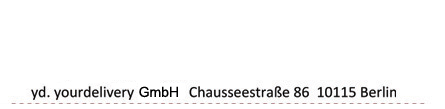
\includegraphics[scale=0.5]{../pdf/address.jpg}}

\renewcommand{\headrulewidth}{0pt}

% footer
\fancyfoot[L]{}
\fancyfoot[C]{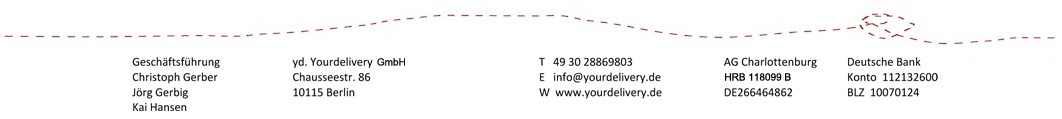
\includegraphics[scale=0.5]{../pdf/footer_only.jpg}}
%\fancyfoot[C]{
\includegraphics[scale=0.6]{../pdf/footer.eps}}
\fancyfoot[R]{}


%-------------------------------- content
\begin{document}
	
    % Bestellinformationen
		\begin{tabular}{v{0.5\textwidth}w{0.3\textwidth}r}
		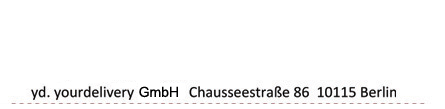
\includegraphics[scale=0.5]{../pdf/address.jpg}

		         	       	\textrm{sportme GmbH}\\
		         		\textrm{Chauseestr. 86}\\
				\textrm{10115 Berlin}\\
				\textrm{Deutschland}\\
				
				& \\
		\end{tabular}
                %add all members from group

                %add all members who will share their budget
            
            	\vspace{1.5cm}
	
		\begin{tabular}{v{0.7\textwidth}r}
				\begin{large}
					Gutschrift: \textbf{GUT-94589489}
				\end{large}
				&  Berlin, den {\today} \\ \\ \\
				Leistungszeitraum:		& 15.04.2009 - 31.12.2009\\ \\
				
				
				
				Netto gesamt:		& \EUR{120,00} \\
				\hline
				Netto  7 \%:		& \EUR{20,00} \\
				Netto 19 \%:		& \EUR{100,00} \\
				MwSt 7 \%:		& \EUR{1,40} \\
				MwSt 19 \%:		& \EUR{19,00} \\
				  \hline
				Umsatz Brutto:			& \EUR{140,40} \\
				  \hline  \hline
				
		\end{tabular}
		\\ \\ \\
		
		Vom Kunden bereits bei Ihnen bar bezahlt: \EUR{60,00}\\ \\
		InVerrechnung mit den bestehenden Forderungen (Provision yourdelivery.de) von \EUR{16,71} aus der offenen Rechnung R-09941-5332555 "uberweisen wir Ihnen auf Ihr Konto:
		\begin{center}
			\begin{tabular}{x{\textwidth}r!}
				\noalign{\hrule height 1.2pt}
				
				\multicolumn{2}{!{\vrule width 1.2pt}x{\textwidth}!{\vrule width 1.2pt}}{\textbf{\EUR{63,25}}}  \\
				\noalign{\hrule height 1.2pt}
			\end{tabular}
		\end{center}
		\vspace{2cm}
				
			
\includegraphics[scale=0.5]{../pdf/unterschrift.jpg}
		
		
		
\end{document}